% Étape Global : toute l'image, sur une carte réduite de moitié (FreeFlow)
% Compiler avec pdflatex (ou Overleaf).
\documentclass[border=10pt]{standalone}
\usepackage[T1]{fontenc}
\usepackage[utf8]{inputenc}
\usepackage[scaled]{helvet}
\renewcommand{\familydefault}{\sfdefault}
\usepackage{sansmath}
\sansmath
\usepackage{amsmath}
\usepackage{tikz}
\usetikzlibrary{arrows.meta}

% couleurs simples
\definecolor{bleu}{HTML}{9CC8F0}    % patchs (N x D)
\definecolor{vert}{HTML}{A8DCA0}    % tokens réduits (N/4 x D)
\definecolor{jaune}{HTML}{FFE27A}   % attention
\definecolor{rouge}{HTML}{F4A6A6}   % G, retour à N x D
\definecolor{gris}{HTML}{CCCCCC}
\definecolor{grisclair}{HTML}{F2F2F2}
\definecolor{noir}{HTML}{222222}

\tikzset{
  th/.style={font=\fontsize{14}{16}\selectfont\bfseries, text=black, inner sep=0pt},
  ts/.style={font=\fontsize{12}{14}\selectfont, text=black, inner sep=0pt},
  tm/.style={font=\fontsize{13}{15}\selectfont, text=black, inner sep=0pt},
  op/.style={font=\fontsize{16}{18}\selectfont, text=black, inner sep=0pt},
  fl/.style={noir, line width=1.5pt, -{Stealth[length=7pt]}},
}
\newcommand{\num}[1]{\tikz[baseline=(c.base)]\node[circle,draw=black,line width=0.7pt,inner sep=1pt,font=\fontsize{10}{10}\selectfont\bfseries](c){#1};}
% \grid{x}{y}{lignes}{colonnes}{case}{couleur}
\newcommand{\grid}[6]{%
  \fill[#6] (#1,#2) rectangle ++(#4*#5,#3*#5);
  \ifnum#4>1 \foreach \k in {1,...,\numexpr#4-1\relax} \draw[white, line width=1pt] (#1+\k*#5,#2) -- ++(0,#3*#5); \fi
  \ifnum#3>1 \foreach \k in {1,...,\numexpr#3-1\relax} \draw[white, line width=1pt] (#1,#2+\k*#5) -- ++(#4*#5,0); \fi}

\begin{document}
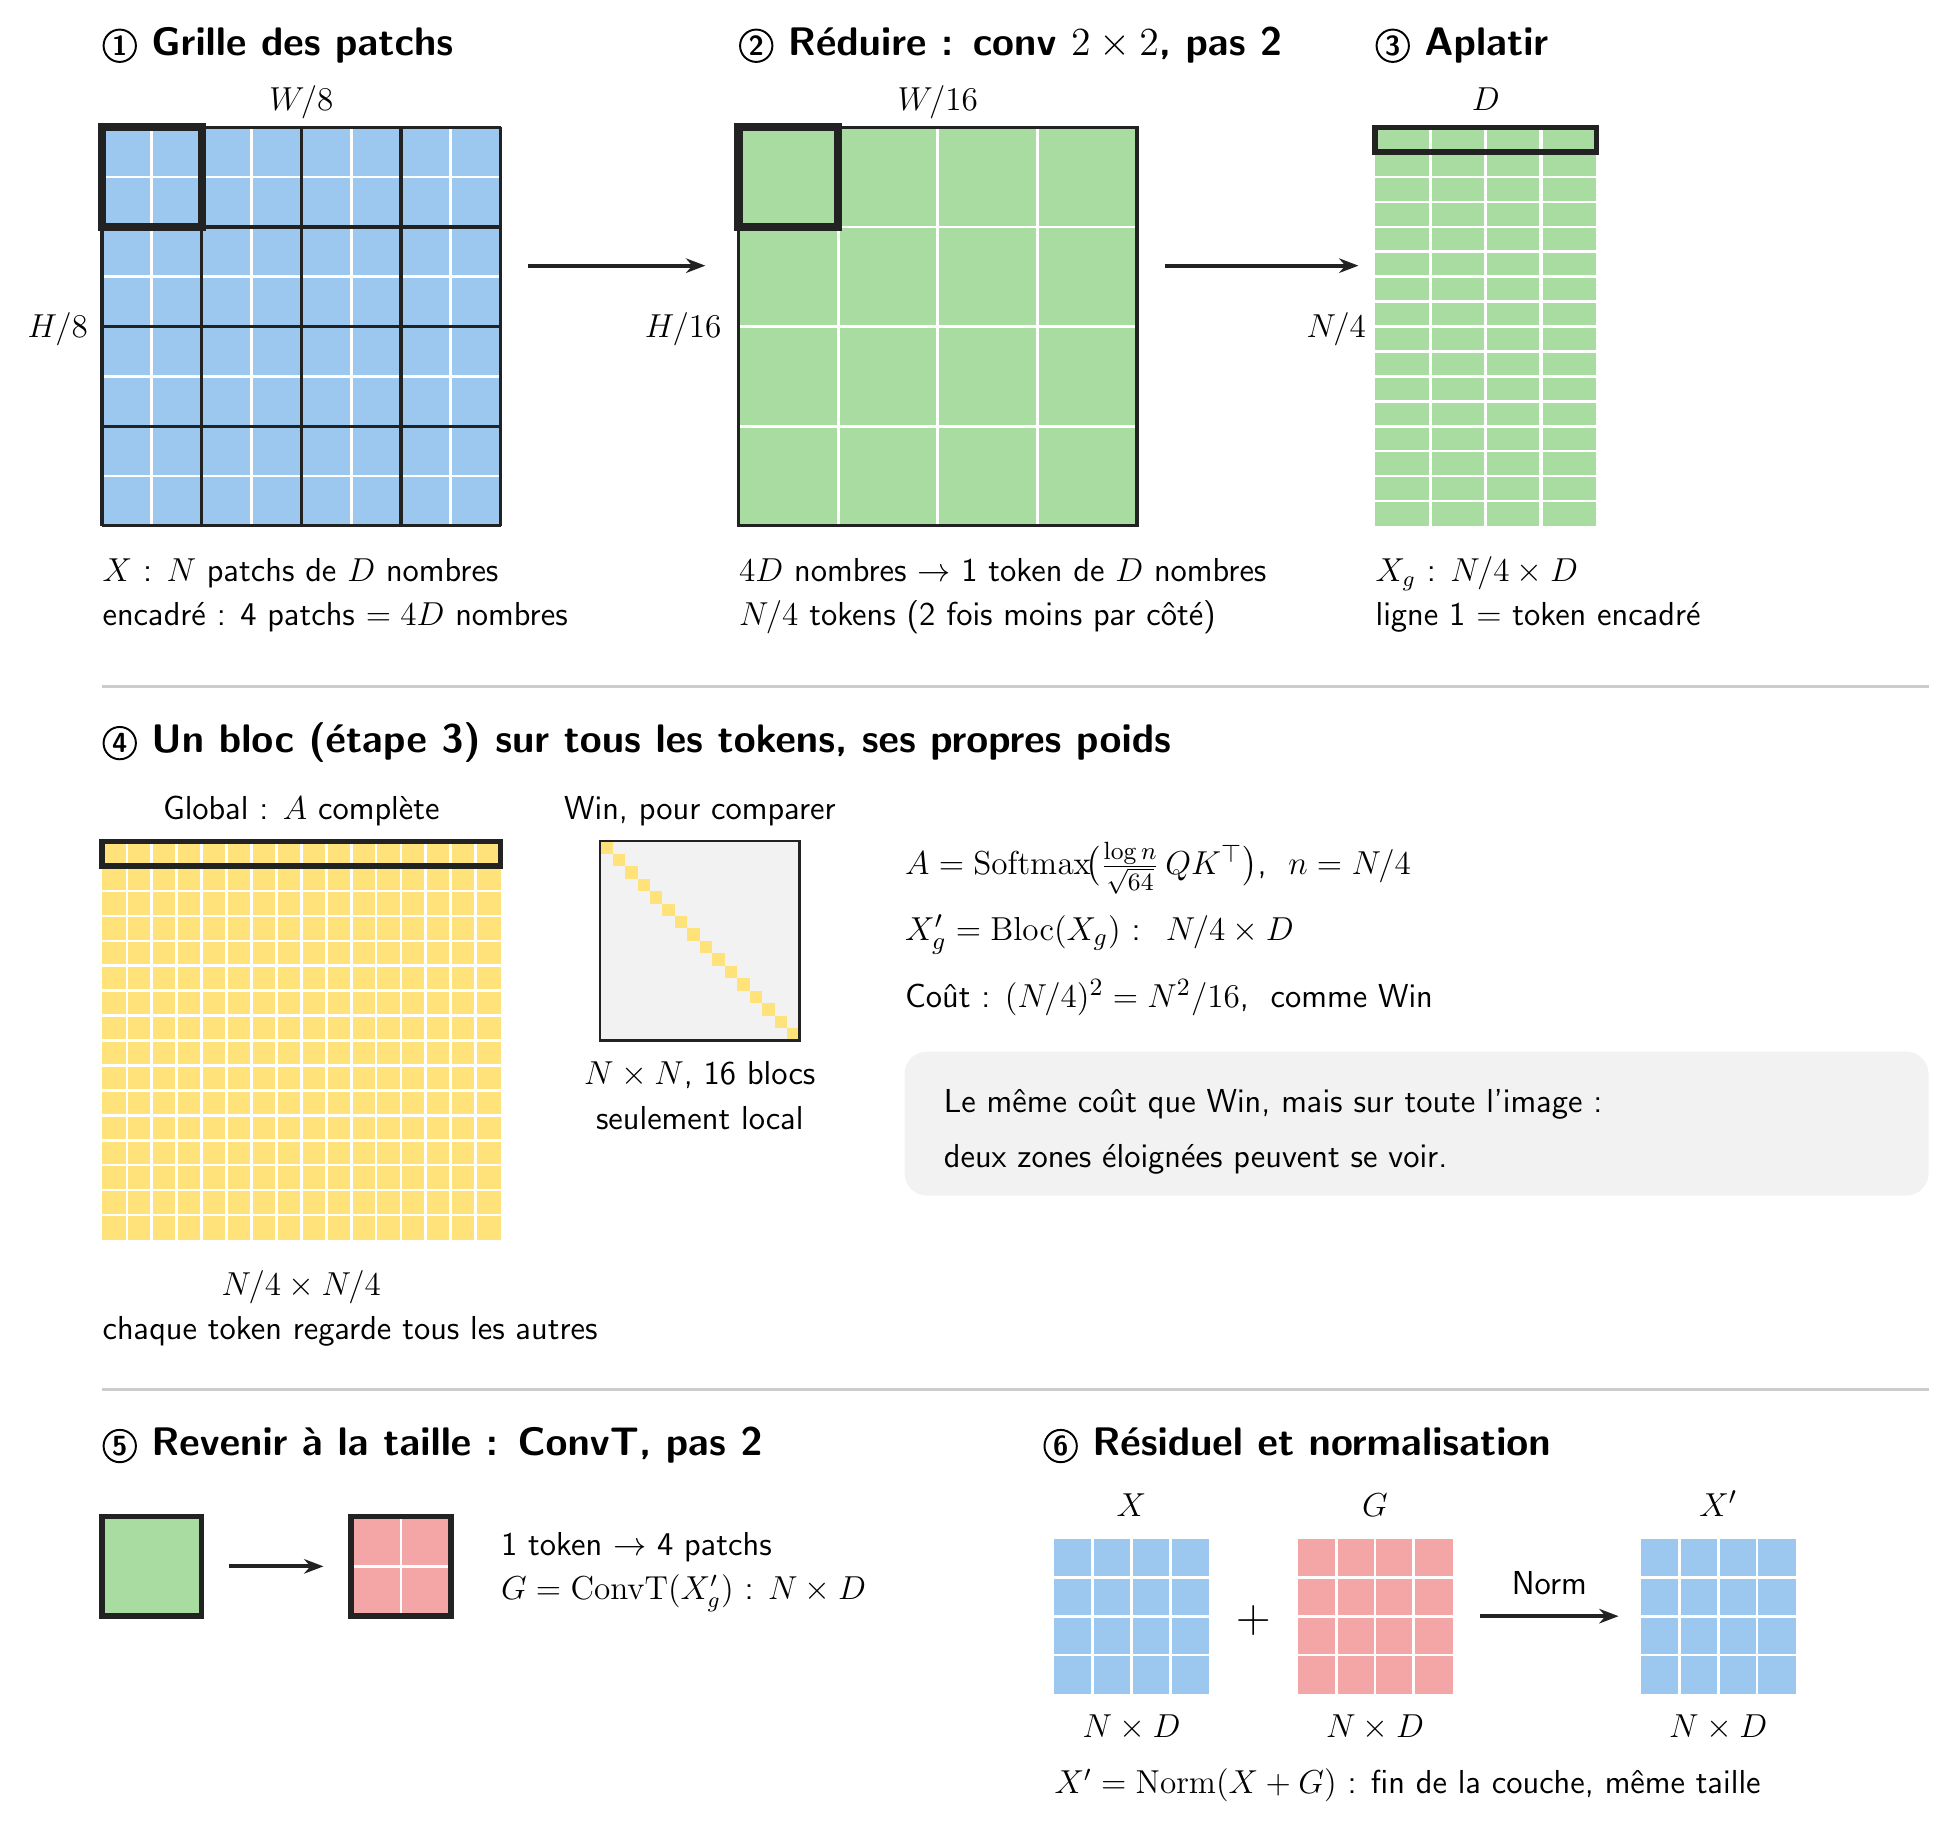
\begin{tikzpicture}[x=1pt, y=-1pt, line join=miter]

% =============== LIGNE 1 : réduire ===============
\node[th, anchor=base west] at (40,24)  {\num{1} Grille des patchs};
\node[th, anchor=base west] at (270,24) {\num{2} Réduire : conv $2 \times 2$, pas 2};
\node[th, anchor=base west] at (500,24) {\num{3} Aplatir};

% 1. grille (H/8) x (W/8), groupes de 2 x 2
\grid{40}{50}{8}{8}{18}{bleu}
\foreach \k in {0,...,4} {
  \draw[noir, line width=1.2pt] (40+36*\k,50) -- ++(0,144);
  \draw[noir, line width=1.2pt] (40,50+36*\k) -- ++(144,0);
}
\draw[noir, line width=3pt] (40,50) rectangle (76,86);
\node[ts, anchor=base] at (112,44) {$W/8$};
\node[ts, anchor=base] at (24,126) {$H/8$};
\node[ts, anchor=base west] at (40,214) {$X$ : $N$ patchs de $D$ nombres};
\node[ts, anchor=base west] at (40,230) {encadré : 4 patchs $= 4D$ nombres};

\draw[fl] (194,100) -- (258,100);

% 2. carte réduite (H/16) x (W/16)
\grid{270}{50}{4}{4}{36}{vert}
\draw[noir, line width=1.2pt] (270,50) rectangle (414,194);
\draw[noir, line width=3pt] (270,50) rectangle (306,86);
\node[ts, anchor=base] at (342,44) {$W/16$};
\node[ts, anchor=base] at (250,126) {$H/16$};
\node[ts, anchor=base west] at (270,214) {$4D$ nombres $\rightarrow$ 1 token de $D$ nombres};
\node[ts, anchor=base west] at (270,230) {$N/4$ tokens (2 fois moins par côté)};

\draw[fl] (424,100) -- (494,100);

% 3. Xg : N/4 x D
\fill[vert] (500,50) rectangle (580,194);
\foreach \x in {520,540,560} \draw[white, line width=1.2pt] (\x,50) -- (\x,194);
\foreach \k in {1,...,15} \draw[white, line width=1pt] (500,50+9*\k) -- (580,50+9*\k);
\draw[noir, line width=2pt] (500,50) rectangle (580,59);
\node[ts, anchor=base] at (540,44) {$D$};
\node[ts, anchor=base] at (486,126) {$N/4$};
\node[ts, anchor=base west] at (500,214) {$X_g$ : $N/4 \times D$};
\node[ts, anchor=base west] at (500,230) {ligne 1 = token encadré};

% =============== LIGNE 2 : attention sur tout ===============
\draw[gris, line width=1pt] (40,252) -- (700,252);
\node[th, anchor=base west] at (40,276) {\num{4} Un bloc (étape 3) sur tous les tokens, ses propres poids};

% Global : A pleine
\node[tm, anchor=base] at (112,300) {Global : $A$ complète};
\grid{40}{308}{16}{16}{9}{jaune}
\draw[noir, line width=2pt] (40,308) rectangle (184,317);
\node[ts, anchor=base] at (112,472) {$N/4 \times N/4$};
\node[ts, anchor=base west] at (40,488) {chaque token regarde tous les autres};

% comparaison : Win
\node[tm, anchor=base] at (256,300) {Win, pour comparer};
\fill[grisclair] (220,308) rectangle (292,380);
\foreach \k in {0,...,15} \fill[jaune] (220+4.5*\k,308+4.5*\k) rectangle ++(4.5,4.5);
\draw[noir, line width=0.8pt] (220,308) rectangle (292,380);
\node[ts, anchor=base] at (256,396) {$N \times N$, 16 blocs};
\node[ts, anchor=base] at (256,412) {seulement local};

\node[tm, anchor=base west] at (330,320) {$A = \mathrm{Softmax}\!\big(\tfrac{\log n}{\sqrt{64}}\, Q K^{\top}\big)$, \ $n = N/4$};
\node[tm, anchor=base west] at (330,344) {$X'_g = \mathrm{Bloc}(X_g)$ : \ $N/4 \times D$};
\node[tm, anchor=base west] at (330,368) {Coût : $(N/4)^2 = N^2/16$, \ comme Win};
\fill[grisclair, rounded corners=8pt] (330,384) rectangle (700,436);
\node[tm, anchor=base west] at (344,406) {Le même coût que Win, mais sur toute l'image :};
\node[tm, anchor=base west] at (344,426) {deux zones éloignées peuvent se voir.};

% =============== LIGNE 3 : revenir et ajouter ===============
\draw[gris, line width=1pt] (40,506) -- (700,506);
\node[th, anchor=base west] at (40,530) {\num{5} Revenir à la taille : ConvT, pas 2};
\node[th, anchor=base west] at (380,530) {\num{6} Résiduel et normalisation};

% ConvT : 1 token -> 2 x 2 patchs
\grid{40}{552}{1}{1}{36}{vert}
\draw[noir, line width=2pt] (40,552) rectangle (76,588);
\draw[fl] (86,570) -- (120,570);
\grid{130}{552}{2}{2}{18}{rouge}
\draw[noir, line width=2pt] (130,552) rectangle (166,588);
\node[ts, anchor=base west] at (184,566) {1 token $\rightarrow$ 4 patchs};
\node[ts, anchor=base west] at (184,582) {$G = \mathrm{ConvT}(X'_g)$ : $N \times D$};

% X' = Norm(X + G)
\node[tm, anchor=base] at (412,552) {$X$};
\grid{384}{560}{4}{4}{14}{bleu}
\node[op, anchor=base] at (456,594) {$+$};
\node[tm, anchor=base] at (500,552) {$G$};
\grid{472}{560}{4}{4}{14}{rouge}
\draw[fl] (538,588) -- (588,588);
\node[ts, anchor=base] at (563,580) {Norm};
\node[tm, anchor=base] at (624,552) {$X'$};
\grid{596}{560}{4}{4}{14}{bleu}
\node[ts, anchor=base] at (412,632) {$N \times D$};
\node[ts, anchor=base] at (500,632) {$N \times D$};
\node[ts, anchor=base] at (624,632) {$N \times D$};
\node[ts, anchor=base west] at (384,652) {$X' = \mathrm{Norm}(X + G)$ : fin de la couche, même taille};

\end{tikzpicture}
\end{document}
